\documentclass{report}
\usepackage[utf8]{inputenc}
\usepackage{amsmath}
\usepackage{graphicx}

\title{Øvelser - Fibonnaci Heaps}
\author{André Oskar Andersen (wpr684)}
\date{\today}

\begin{document}
\maketitle

\section*{19.2 - 1}
\textbf{Show the Fibonacci heap that results from calling} \texttt{FIB-HEAP-EXTRACT-MIN} \textbf{on the Fibonacci heap shown in figure 19.4(m)} \\
Svar: \\
\begin{center}
    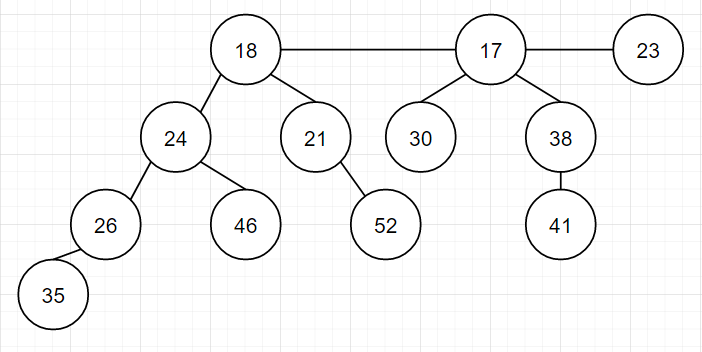
\includegraphics[width = 7 cm]{../entities/19_2_1.png}
\end{center}

\section*{19-3 (a)}
\textbf{The operation} \texttt{FIB-HEAP-CHANGE-KEY(H, x, k)} \textbf{changes the key of node $x$ to the value $k$. Give an efficient implementation, and analyze the amortized running time of ypur implementation for the cases in which $k$ is greater than or less than $x.key$}
Svar:
\begin{verbatim}
    FIB-HEAP-CHANGE-KEY(H, x, k):
    if (k < x.key):
        FIB-HEAP-DECREASE-KEY(H, x, k)
    elif (k > x.key):
        DELETE(H, x)
        INSERT(H, k)
\end{verbatim}
For the first case, the running time is $O(1)$. For the second case, the running time is $O(\lg n)$

\section*{19.4 - 1}
\textbf{Professor Pinocchio claims that the height of an nn-node Fibonacci heap is $O(\lg n)$. Show that the professor is mistaken by exhibiting, for any positive integer nn, a sequence of Fibonacci-heap operations that creates a Fibonacci heap consisting of just one tree that is a linear chain of nn nodes.} \\
Svar: \\
Insert 33 numbers, in which at least two numbers are less than the root of chain, then extract-min. The smallest newly inserted number will be extracted and the remaining two numbers will form a heap whose degree of root is 11, and since the root of the heap is less than the old chain, the chain will be merged into the newly created heap. Finally we should delete the node which contains the largest number of the 3 inserted numbers.

\end{document}